%%%%%%%%%%%%%%%%%%%%%%%%%%%%%%%%%%%%%%%%%%%%%%%%%%%%%%%%%%%%%%%%%%%
%%% Documento LaTeX 																						%%%
%%%%%%%%%%%%%%%%%%%%%%%%%%%%%%%%%%%%%%%%%%%%%%%%%%%%%%%%%%%%%%%%%%%
% Título:		Capítulo 3
% Autor:  	Ignacio Moreno Doblas
% Fecha:  	2014-02-01, actualizado 2019-11-11
% Versión:	0.5.0
%%%%%%%%%%%%%%%%%%%%%%%%%%%%%%%%%%%%%%%%%%%%%%%%%%%%%%%%%%%%%%%%%%%
% !TEX root = A0.MiTFG.tex

\chapterbegin{Fundamentos teóricos}
\label{chp:App}
\minitoc

\section{Introducción a los esquemas de señalización}
%Hablar sobre qué són los esquemas de señalización y cual es su función principal. comentar
%los esquemas (alternos,cancelación,4ppm,4ippm y pwm) y por qué se han elegido o descartado.
%Decir que no son los esquemas del estándar y que se han elegido para investigar sus ventajas e inconvenientes. 

En el ámbito de la comunicación existen múltiples esquemas de codificación digital con diferentes propiedades como 
probabilidad de bit, ciclo de trabajo, ancho de banda, etc. A la hora de estudiar un esquema de codificación para hacer 
su elección hay que tener en cuenta tres aspectos fundamentales, que son:
\begin{itemize}
    \item Flickering: se define como el cambio de la luz provocado por la conmutación entre encendido 
y apagado (1 y 0) en intervalos muy cortos. 
Estos parpadeos, si se producen a una velocidad perceptible por el ojo humano, pueden llegar a ser molestos y causar dolor. 
    \item Rendimiento óptico.
    \item La capacidad para controlar la atenuación o el dimming, provocado por por la variación de la intensidad de la luz, 
    en esquemas de codificación con ancho de pulso de la señal variable. 
\end{itemize} 

El estándar de comunicaciones por luz visible IEEE 802.15.7 usa como esquema de señalización la codificación Manchester. 
Continuando con el estudio de los esquemas de señalización,
a continuación, se van a desarrollar otras opciones de esquemas de codificación con características diferentes
para estudiar su eficacia e impacto en las comunicaciones por luz visible.
Los esquemas a desarrollar son codificación por pulsos alternos, cancelación de pulsos y 4-ppm. También se hará una 
comparativa de 4-ppm frente a Inverse 4-ppm para comparar sus prestaciones y el efecto de transmitir mayor cantidad 
de ``unos'' que de ``ceros''.

Es importante destacar que en un primer momento también se planteó el desarrollo de codificación 4-PWM pero se descartó su 
implementación debido a su escasa capacidad para controlar el dimming. Esto provocaba que la intensidad de la luz 
fluctuara mucho a lo largo de una transmisión siendo perceptible y molesto para el ojo humano.

\section{Pulsos alternos}
% Comentar teóricamente en que consiste este esquema (miller pero con una opción menos y alternando).
% Y que apenas está implementado y desarrollado en ningún sitio.
El primer esquema de codificación desarrollado es pulsos alternos. Este esquema 
se puede considerar como una versión de la codificación Manchester pero
añadiendo tiempos de silencio. Estos tiempos de silencio añadidos en la transmisión
se emplean para diseñar formatos OOK con memoria mediante el uso de de la alternancia de
posición de pulsos. Lo que proporciona una mejora notable en el rendimiento y una 
configuración del espectro favorable. 
Este formato de pulsos alternos tiene un ciclo de trabajo bajo, lo que provoca que esta 
codificación sea ventajosa en términos de modulación de intensidad y detección directa. 
En este esquema, utilizamos los tiempos de silencio y los pulsos alternos para
modificar las estadísticas de la secuencia de amplitud con respecto a las estadísticas de 
la secuencia de mensajes.

De esta manera, el bit de información '0' siempre se codifica con la ausencia de pulso 
'00', mientras que el bit '1' se representa con un pulso que va variando su posición con
cada transmisión del '1'. Gracias a aplicar este esquema, se reduce el número de pulsos 
transmitidos en otros esquemas de señalización como Manchester o Miller.

%Dibujar y comentar el diagrama de trellis de este esquema
La figura \ref{trellis_alternos} representa el diagrama de Trellis de este esquema de 
codificación tal y como se ha descrito anteriormente. Este modelo consiste en dos estados,
imprescindibles para la alternancia de pulsos. Lo más destablace del diagrama es que 
siempre que se codifica un '0' nos mantenemos en el mismo estado y siempre que se 
codifca un '1' cambiamos de estado para realizar la alternancia de pulsos. Será en el 
momento de cambio de estado cuando codificaremos el pulso correspondiente que dependerá 
del estado al que se transicione.
\vspace{1cm}

\begin{figure}[ht]
    \centering
    %   TRELLIS PULSOS ALTERNOS

\tikzstyle{state}=[shape=circle,draw=blue!50,fill=blue!20,inner sep=2pt]
\def\desp{1.5}%
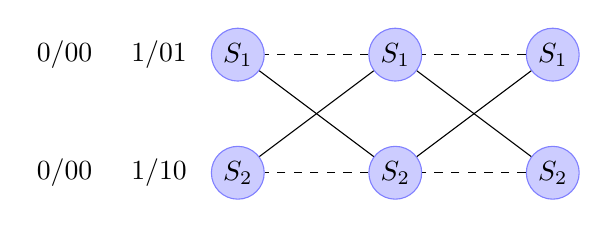
\begin{tikzpicture}[]
% 1st column
\draw (0,\desp) node[name=s1_1,state] {$S_1$} node[xshift=-2.2cm]{$0/00$}node[xshift=-1cm]{$1/01$};
\draw (0,0) node[name=s2_1,state] {$S_2$} node[xshift=-2.2cm]{$0/00$}node[xshift=-1cm]{$1/10$};
% 2nd column

\node[state] (s1_2) at (2,\desp) {$S_1$}
    edge[dashed] (s1_1)
    edge[thin] (s2_1);
\node[state] (s2_2) at (2,0) {$S_2$}
    edge[thin] (s1_1)
    edge[dashed] (s2_1);

% 3rd column

\node[state] (s1_3) at (4,\desp) {$S_1$}
    edge[dashed] (s1_2)
    edge[thin] (s2_2);
\node[state] (s2_3) at (4,0) {$S_2$}
    edge[thin] (s1_2)
    edge[dashed] (s2_2);
\end{tikzpicture}

\hspace{1cm}--------- $1$ ---------

\hspace{1cm} - - - - - $0$ - - - - -

    \caption{\small{Diagrama de Trellis de la codificación pulsos alternos.}}
    \label{trellis_alternos}%
\end{figure}

El esquema de señalización resultante se muestra en la figura \ref{codificacion_alternos}.

%% INSERTAR FIGURA DE LA CODIFICACIÓN
\begin{figure}[ht]
    \centering
    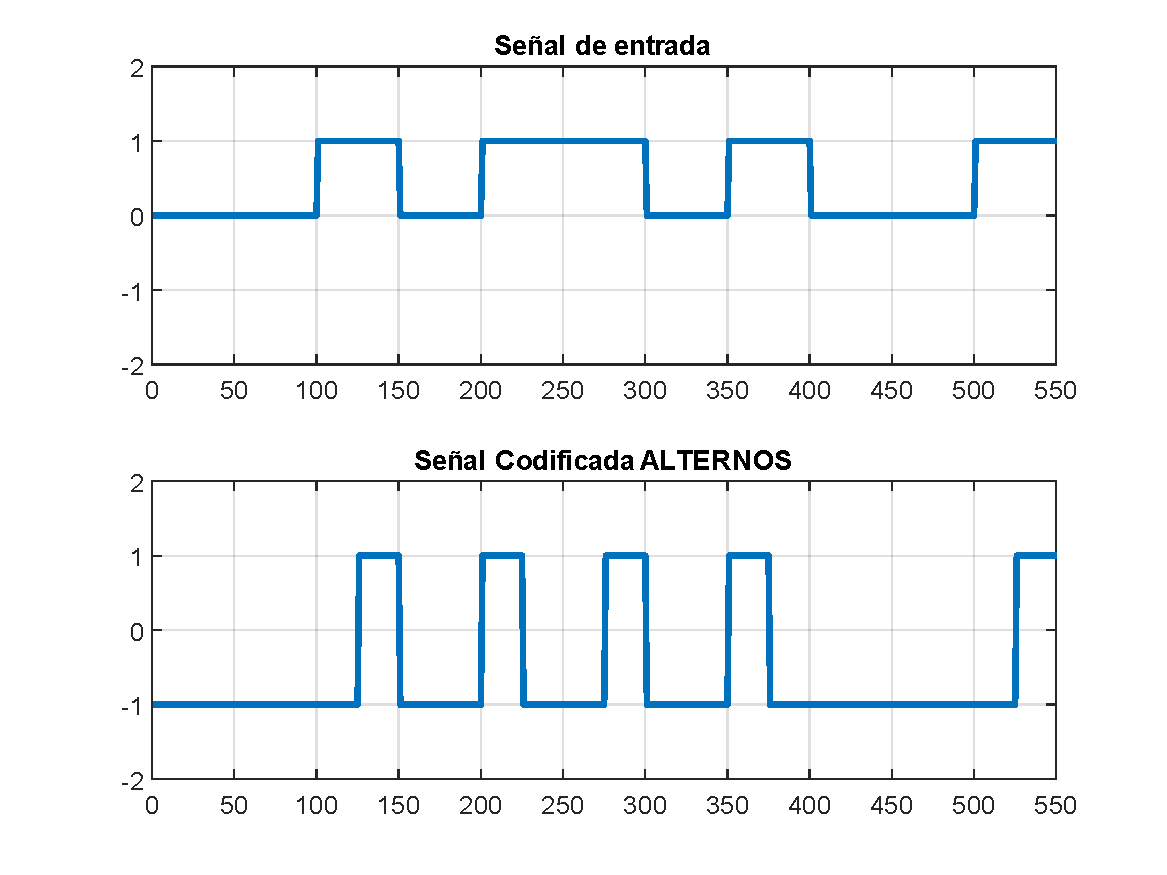
\includegraphics[scale=0.5]{./figuras/CodificadaAlternos.pdf}
    \caption{\small{Codificación con pulsos alternos.}}
    \label{codificacion_alternos}%
\end{figure}

En dicha figura se observa perfectamente el funcionamiento de este esquema de 
señalización. En la parte superior de la figura se encuentra la trama pseudoaleatoria y 
abajo su codificación en la que se muestra como los pulsos alteran en cada codificación 
de '1' y que siempre se que codifica un '0' hay ausencia de pulsos. Además, la señal 
codificada se encuentra entre -1V y 1V lo que implica que ya está preparada para ser 
transmitida por el canal de luz. La señal codificada trabaja a el doble de frecuencia que 
la señal de entrada ya que hay transiciones rápidas cuando se transmite un pulso al igual
que ocurre con la codificación Manchester que especifica el estándar.

Además, también se observa que el ciclo de trabajo es bajo cuya ventaja, como se ha 
comentado anteriormente, es que proporciona mayor intensidad de iluminación cuando se 
transmite un pulso. Sin embargo, también tiene una desventaja que va ligada al flickering.
Al tranmsitir mayor cantidad de '0' que de '1' el transmisor se encuentra más tiempo 
apagado por lo que el parpadeo es más notable para el ojo humano que en otras 
codificaciones como Manchester o Miller por lo que se necesitará una frecuencia de 
transmisión mayor para este esquema de señalización para que el flickering no sea 
perceptible por el ojo humano y llegue a ser molesto.

% Por qué es un esquema no equiprobable haciendo los cálculos correspondientes.
Este esquema al tener mayor número de '0' que de '1' se convierte en un esquema no 
equiprobable, es decir, en un esquema que no tiene la misma probabilidad de transmitir 
'0' que '1'. Es importante realizar los cálculos correspondientes para conocer la 
probabilidad exacta de cada bit para conocer el ciclo de trabajo y el efecto que 
provoca en el receptor óptico la no equiprobabilidad.
%%%%%%%%%%%%%%%%%%%% FORMULA DE LA PROBABILIDAD %%%%%%%%%%%%%%%%%%%%%%%%%%%%%%%%

% BER 
Se han estudiado sus prestaciones para tener una idea de cómo funciona este esquema. 
El funcionamiento depende del sistema de decisión que se aplique (estos sistemas de 
explican en el apartado 4.6) pero es bueno tener una visión de su tasa de error de bit.
La figura x muestra la tasa de error de bit (BER) en función de la relación señal a ruido
(SNR) de esque esquema de señalización aplicando \textit{soft-decoding} como sistema de 
decisión. 
%%%%%%%%%%%%%%%%%%% FOTO DE BER SOFT-DECODING %%%%%%%%%%%%%%%%%%%%%%%%%%%%%%%%%

Seguidamente, podemos calcular la densidad de potencia espectral (PSD) de la 
codificación propuesta aplicando la siguiente fórmula.
% Calculo del psd en el paper que me pasó Antonio
%%%%%%%%%%%%%%%%%% FORMULA PSD %%%%%%%%%%%%%%%%%%%%%%%%%%%%%%%%

La densidad de potencia espectral obtenida a través de los cálculos
anteriores se muestra en la figura \ref{psd_alternos}
%%%%%%%% FOTO DEL PSD DEL PAPER DE ANTONIO %%%%%%%%%%%%%%%%
\begin{figure}[ht]
    \centering
    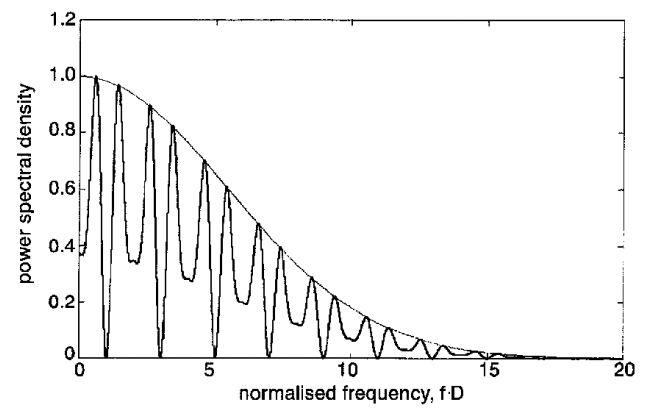
\includegraphics[scale=0.5]{./figuras/psd_alternos.png}
    \caption{\small{Potencia espectral frente a frecuencia normalizada.}}
    \label{psd_alternos}%
\end{figure}

% CONCLUSION 
En definitiva, se ha propuesto una nueva técnica de codificación basada en la 
alternancia de pulsos y en la ausencia de los mismos para modificar las estadísticas de la
secuencia de amplitud con respecto a las estadísticas de la secuencia de mensajes llevando
a una mejora notable para el formato OOK con un rendimiento óptimo.

\section{Cancelación de pulsos}
% Comentar teóricamente en que consiste este esquema (alternos pero eliminando pulsos).
% Y que apenas está implementado y desarrollado en ningún sitio.

Tras el desarrollo de la codificación por pulsos alternos y de haber visto mejora en 
términos de BER, la ventaja proporcionada por modificar las estadísticas de la secuencia
no se explotan completamente ya que la técnica de señalización no presenta ninguna mejora
respecto a la relación de potencia óptica de pico a promedio (PAOPR), y por lo tanto aún
se pueden conseguir mejores resultados. Siguiendo esta línea, para mejorar el pico de 
potencia óptica se trata de disminuir el número de pulsos, centrándose en evitar la 
aparición de más de un pulso de manera consecutiva. 

De esta manera, el bit de información '1' se codifica con la ausencia de pulso '00' 
o con un pulso con su posición modificada, '01'. Mientras que el bit '0' se representa con
ausencia de pulso '00' o con presencia de pulso sin modificar su posición '10'. Gracias
a aplicar esto, se disminuyen los números de pulsos de una manera bastante notable. 

%EXPLICAR EL TRELLIS
La figura \ref{trellis_cancelacion} representa el diagrama de Trellis de este esquema
de codificación tal y como se ha descrito anteriormente. Este modelo consiste en tres 
estados, donde cada estado es imprescindible para saber como codificar el dato.
Lo más importante del trellis es que el primer '1' que se codifica después de un '0'
siempre se codifica como ausencia de pulso ('00') y que siempre que el bit de dato
es un '0' se transiciona al estado S1 para volver a empezar y codificar el primer '1'
como ausencia de pulso. También se observa que después de codificar el primer '1' es 
cuando se produce el pulso con su posición modificada si se codifica otro '1' o el 
pulso con su posición sin modificar si se codifica un '0'.
Hay que destacar que el estado S3 funciona exactamente igual que el estado S1 pero,
sin embargo, es necesario por la naturaleza de los diagramas de Trellis o de Markov, 
ya que no es apropiado que se transicione al mismo estado independientemente del bit 
que se codifique.
\vspace{1cm}

\begin{figure}[ht]
    \centering
    %CANCELACION
\tikzstyle{state}=[shape=circle,draw=blue!50,fill=blue!20,inner sep=2pt]
\def\desp{1.5}%
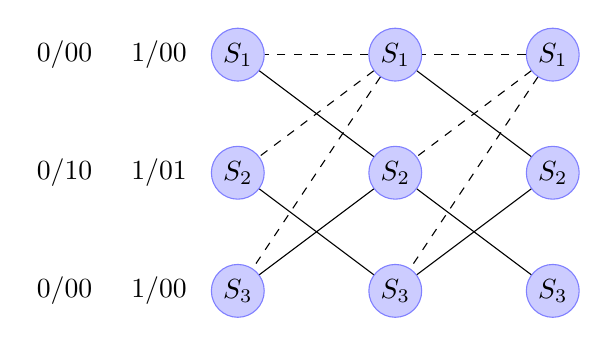
\begin{tikzpicture}[]
% 1st column
\draw (0,3*\desp) node[name=s1_1,state] {$S_1$} node[xshift=-2.2cm]{$0/00$}node[xshift=-1cm]{$1/00$};
\draw (0,2*\desp) node[name=s2_1,state] {$S_2$} node[xshift=-2.2cm]{$0/10$}node[xshift=-1cm]{$1/01$};
\draw (0,\desp) node[name=s3_1,state] {$S_3$} node[xshift=-2.2cm]{$0/00$}node[xshift=-1cm]{$1/00$};

% 2nd column

\node[state] (s1_2) at (2,3*\desp) {$S_1$}
    edge[dashed] (s1_1)
    edge[dashed] (s2_1)
    edge[dashed] (s3_1);
\node[state] (s2_2) at (2,2*\desp) {$S_2$}
    edge[thin] (s1_1)
    edge[thin] (s3_1);
\node[state] (s3_2) at (2,\desp) {$S_3$}
    edge[thin] (s2_1);

% 3d column

\node[state] (s1_3) at (4,3*\desp) {$S_1$}
    edge[dashed] (s1_2)
    edge[dashed] (s2_2)
    edge[dashed] (s3_2);
\node[state] (s2_3) at (4,2*\desp) {$S_2$}
    edge[thin] (s1_2)
    edge[thin] (s3_2);
\node[state] (s3_3) at (4,\desp) {$S_3$}
    edge[thin] (s2_2);


\end{tikzpicture}

\hspace{1cm}--------- $1$ ---------

\hspace{1cm}- - - - - $0$ - - - - -
%\line(1,0){2cm}  $1$ \line(1,0){2cm}


% 1 linea continua, 0 linea discontinua
    \caption{\small{Diagrama de Trellis de la codificación cancelación de pulsos.}}
    \label{trellis_cancelacion}%
\end{figure}

El esquema de señalización resultante se muestra en la figura \ref{codificación_cancelacion},
donde se puede observar una mejora del 50\% en PAOPR. Ya que este formato asegura un 
período mínimo de tiempo sin transiciones consecutivas.

%% INSERTAR FIGURA DE LA CODIFICACIÓN
\begin{figure}[ht]
    \centering
    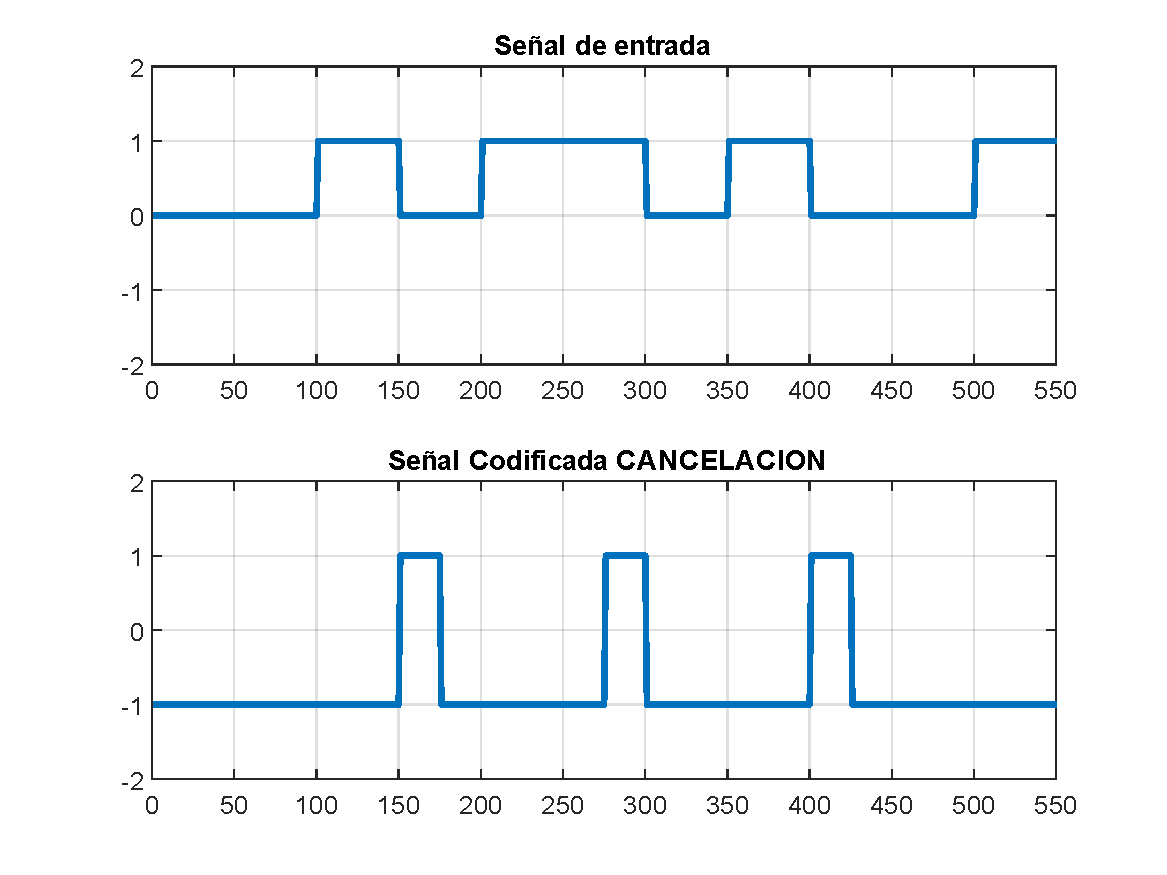
\includegraphics[scale=0.6]{./figuras/CodificadaCancelacion.pdf}
    \caption{\small{Codificación con cancelación de pulsos.}}
    \label{codificación_cancelacion}%
\end{figure}

Además, en dicha figura, se puede apreciar el funcionamiento de este esquema de señalización 
ya que se comprueba que predomina la ausencia de pulsos. En la parte superior de la figura 
se encuentra la trama pseudoaleatoria y abajo su codificación. También se 
observa como la entrada es una señal digital (0 y 1) y como la codificada se encuentra
entre [-1,1] que es el rango de transmisión por el canal de luz.

En este esquema de codificación, la señal codificada tiene el doble de frecuencia de 
trabajo ya que, al igual que otros esquemas como pulsos alternos o Manchester, hay 
transiciones rápidas entre '0' y '1'. 

En la figura también se observa que el ciclo de trabajo de esta codificación es 
bajo porque hay pocos pulsos. Esto provoca dos efectos.
\begin{itemize}
    \item Flickering: al transmitir mayor número de '0' que de '1' la fuente transmisora
        se encuentra más tiempo apagada que encendida. Esto implica que, a la misma 
        frecuencia de transmisión que otros esquemas de codificación, el flickering en 
        cancelación de pulsos sea mayor ya que es uno de los esquemas que mayor 
        diferencia de probabilidad de bits presenta.
    \item Potencia óptica: la ventaja de transmitir pocos pulsos es que estos se pueden 
        transmitir con mayor potencia ya que el transmisor está la mayor parte del tiempo
        sin transmitir. 
\end{itemize}

% Por qué es un esquema no equiprobable haciendo los cálculos correspondientes.
Como se ha explicado anteriormente, este esquema prioriza la ausencia de pulsos por
lo que también es un esquema no equiprobable (no tiene la misma probabilidad de '0'
que de '1'), aunque en mayor medida que en pulsos
alternos ya que en este hay mayor presencia de '0'. Para saber cuales son sus 
probabilidades exactas hay que realizar los cálculos correspondientes. Este cálculo es 
imprescindible para, además de conocer el ciclo de trabajo, conocer el efecto que 
produce en el receptor de luz.
%%%%%%%%%%%%%%%%%%%% FORMULA DE LA PROBABILIDAD %%%%%%%%%%%%%%%%%%%%%%%%%%%%%%%%

Al igual que para pulsos alternos, se han estudiado sus prestaciones en función de varios 
sistemas de decisión. Estos sistemas se explicarán en el apartado 4.6 pero es oportuno 
tener una referencia de su tasa de error de bit para tener una idea inicial de sus 
prestaciones. Para ello, la figura x muestra la tasa de error de bit de este esquema
para una trama pseudoaleatoria aplicando \textit{soft-decoding} como sistema de decisión. 
%%%%%%%%%%%%%%%%%%% FOTO DE BER SOFT-DECODING %%%%%%%%%%%%%%%%%%%%%%%%%%%%%%%%%

A continuación, podemos calcular la densidad de potencia espectral (PSD) de la 
codificación propuesta aplicando la siguiente fórmula.
% Calculo del psd en el paper que me pasó Antonio
%%%%%%%%%%%%%%%%%% FORMULA PSD %%%%%%%%%%%%%%%%%%%%%%%%%%%%%%%%

Por consiguiente, la densidad de potencia espectral obtenida a través de los cálculos
anteriores se muestra en la figura \ref{psd_cancelación}.

\begin{figure}[ht]
    \centering
    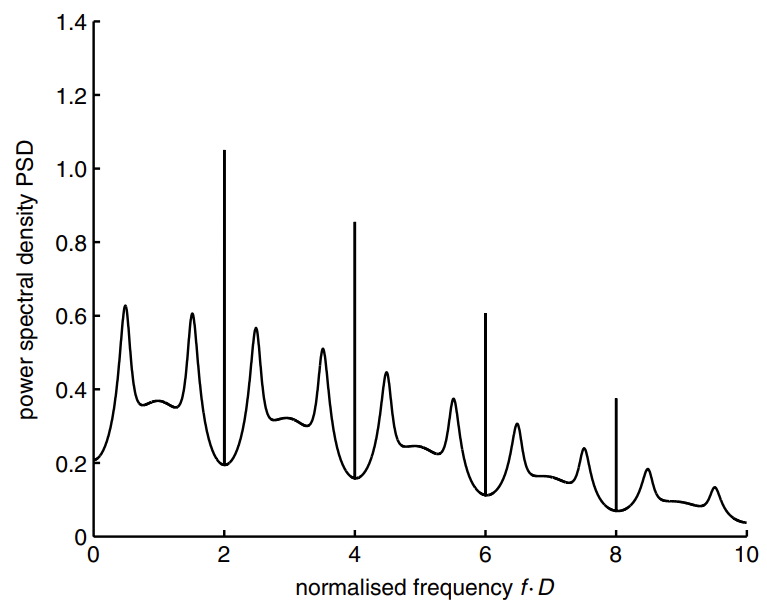
\includegraphics[scale=0.5]{./figuras/psd_cancelacion.png}
    \caption{\small{Potencia espectral frente a frecuencia normalizada.}}
    \label{psd_cancelación}%
\end{figure}


% CONCLUSION 
En conclusión, este esquema de codificación propuesto basado en la ausencia de pulsos
mejora notablemente la codificación de la señal.
El aumento de los tiempos de silencio se utilizan para modificar las estadísticas de
la secuencia de amplitud con respecto a las estadísticas de la
secuencia de mensajes, lo que permite el aumento de la PAOPR,
que es una característica favorable en enlaces ópticos. De esta manera se 
obtiene una buena compensación entre rendimiento y complejidad requerida.

\section{4-PPM}
% Explayarme mucho más porque hay mucha más información.
% Comentar teóricamente en que consiste este esquema.
Este esquema de señalización 
proviene de la modulación por posición de pulso (PPM).
La modulación por posición de pulso es un modo de codificación en el que M bits son 
codificados para transmitir un pulso de duración $ T_C = T/2^M $ en una de las $ 2^M $ 
posiciones posibles en un intervalo de tiempo de T segundos, que es la duración del símbolo.
Este esquema se repite cada T segundos, por lo tanto, la tasa de transmisión es $M/T$ bits 
por segundo. La
atenuación de la luz se lleva a cabo mediante la reducción de la potencia transmitida de 
acuerdo con el
porcentaje requerido de atenuación.
Uno de los esquemas sugeridos es el esquema 4-PPM y es el que se desarrolla en este trabajo.
Gracias a estos esquemas, como la potencia media es constante, se evitan las variaciones 
en la intensidad, pero para ello se necesita una buena sincronización.

En este esquema se codifica cada pareja de bits
por la posición de pulso en cuatro posiciones posibles como se aprecia en la figura
\ref{bits4ppm}.

\begin{figure}[ht]
    \centering
    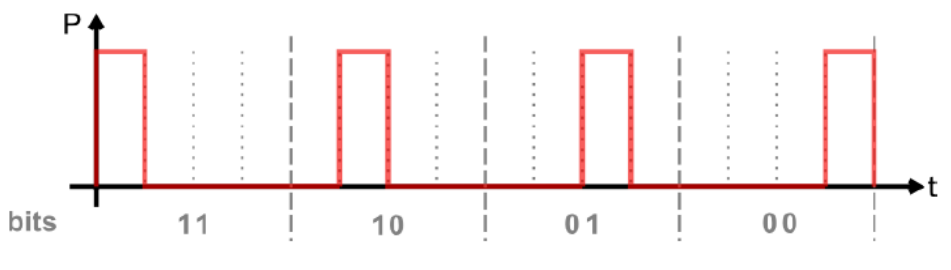
\includegraphics[scale=0.5]{./figuras/opciones4PPM.png}%referencia del paper estado arte
    \caption{\small{Pareja de bits con su respectiva codificación.}}
    \label{bits4ppm}%
\end{figure}

El esquema de señalización resultante se muestra en la figura \ref{cod4ppm}
% PUEDE SER BUENO METER LA SEÑAL DE RELOJ EN MEDIO DE LA ENTRADA Y LA CODIFICADA
\begin{figure}[ht]
    \centering
    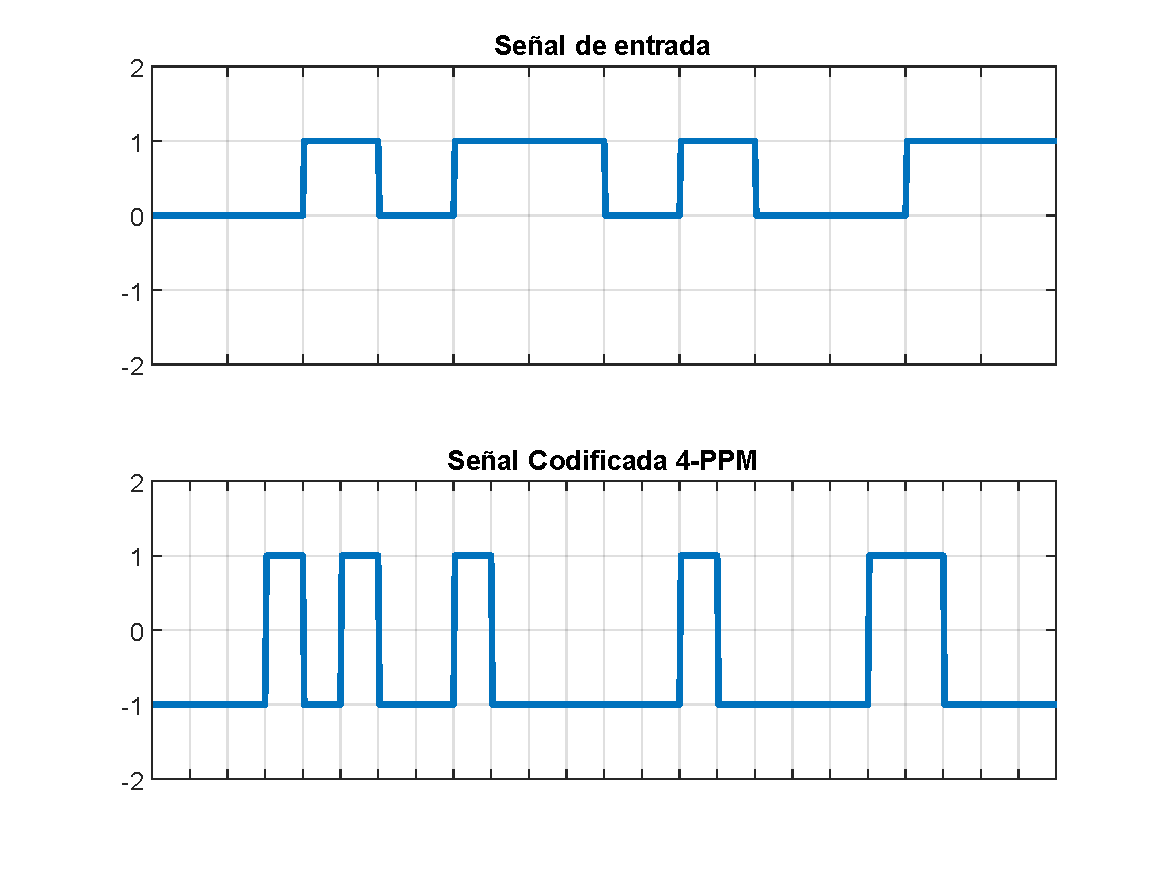
\includegraphics[scale=0.5]{./figuras/CodificadaPPM.pdf}%referencia del paper estado arte
    \caption{\small{Codificación 4-PPM.}}
    \label{cod4ppm}%
\end{figure}


% si encuentro algo hablar sobre cual es su espectro y las diferencias respecto a los del estándar

% Desarrollar por qué es un esquema no equiprobable haciendo los cálculos correspondientes.

% Comentar si se encuentra la ber y sus prestaciones

\section{Comparativa 4-PPM frente a Inverse 4-PPM}
Comparar estos dos esquemas y comentar ventajas e inconvenientes.
%https://ieeexplore.ieee.org/stamp/stamp.jsp?tp=&arnumber=6614862
%https://ieeexplore.ieee.org/stamp/stamp.jsp?tp=&arnumber=567560&tag=1

\section{Sistemas de decisión}
%Hablar sobre las técnicas usadas --> hard-decoding, soft-decoding y algoritmo de Viterbi
%Tener en cuenta el mapeo que se realiza para poner la señal en el rango [-8192,8191]
Hoy en día, una tarea desafiante en la corrección de errores es decodificar las palabras 
de código que se han recibido a través de canales ruidosos. Si no hay errores, es decir, 
las palabras de código encuentran una coincidencia exacta, entonces es fácil decodificar 
los datos. Sin embargo, si no se encuentra una coincidencia, se adoptan diversos mecanismos
de decodificación más complejos. Por este motivo,
en este apartado, se van a describir los diferentes sistemas de decisión para interpretar 
la señal recibida de la mejor manera posible que se han implementado. Para ello, se van a
desarrollar sus características más representativas así como sus ventajas e inconvenientes.

\subsection{Hard-decoding}
El primer sistema de decisión desarrollado es \textit{hard-decoding}. Este sistema es 
el más sencillo de todos y por ello suele ser el que se aplica en la mayoría de sistemas
de comunicación sencillos que no necesitan de alta robustez frente al ruido.

Para su desarrollo es imprescindible fijar un umbral ya que este método compara los 
valores de los pulsos recibidos con el valor del umbral fijado. El valor del umbral se 
determina en la mitad del pulso. Por lo que si el valor del dato es mayor que el valor 
del umbral se interpreta como un '1' y, de lo contrario, se interpreta como un '0'.
La decodificación se realiza siempre igual independientemente de lo cerca que se encuentre 
el valor del dato del umbral.

Es por este motivo que este sistema de decisión es muy poco robusto frente a picos de 
ruido y frente a la inlcusión de componente de continua que pueda modificar y mover 
la amplitud de la señal, provocando que el umbral no se encuentre en la mitad que 
se preveía.

A continuación, se muestra la figura \ref{hard-decoding} que compara el funcionamiento de 
los tres esquemas de codificación desarrollados con el método \textit{hard-decoding}.

\begin{figure}[ht]
    \centering
    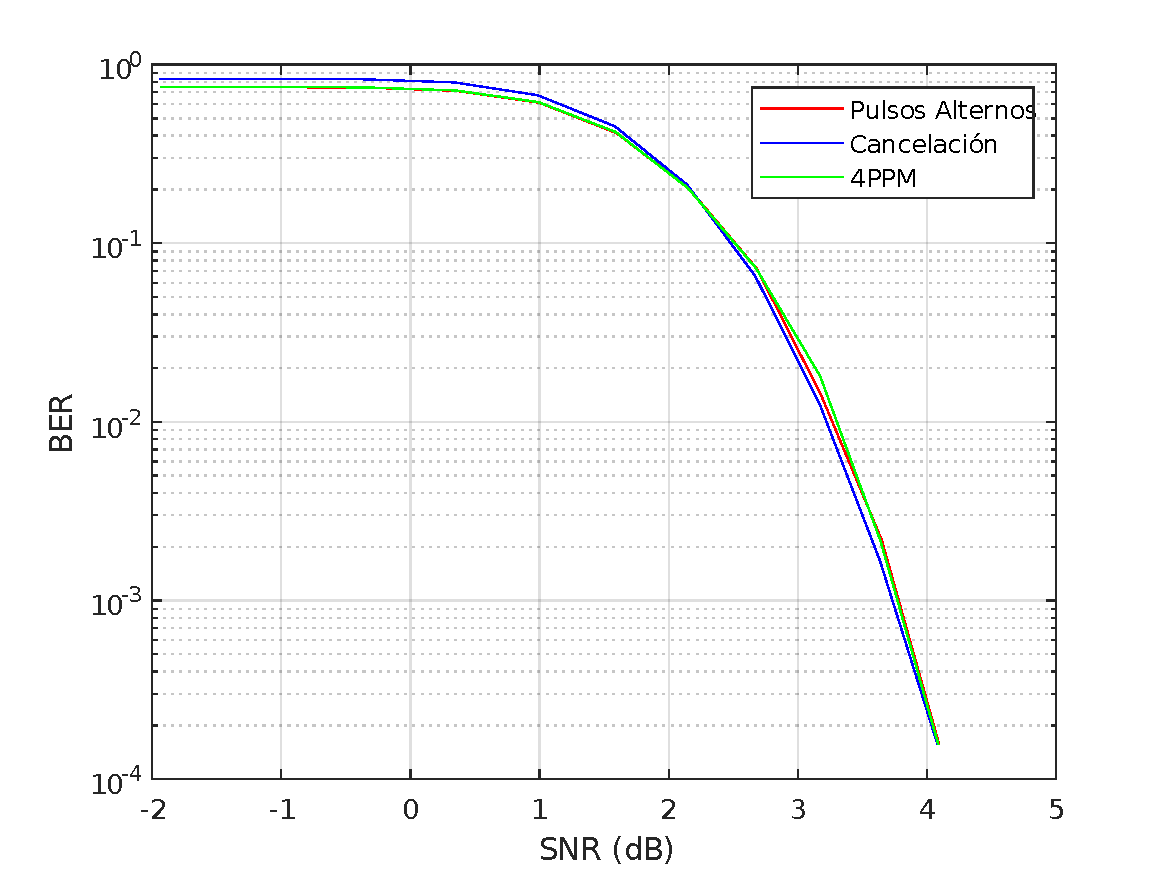
\includegraphics[scale=0.65]{./figuras/Hard.pdf}
    \caption{\small{Sistema \textit{Hard-decoding}.}}
    \label{hard-decoding}%
\end{figure}

En la figura se puede comprobar como, con este sistema, los tres esquemas de señalización 
funcionan esencialmente igual y que, con relaciones señal a ruido bajas (o negativas), la 
tasa de error de bit es alta y no sería aceptable para cualquier sistema de comunicación
por lo que este sistema sólo es apto para comunicaciones directas y cercanas en las que 
la señal se reciba prácticamente perfecta con muy poco ruido.

Tal y como se ha explicado en este apartado, el sistema \textit{hard-decoding} es 
un sistema sencillo y rápido de implementar, sin embargo, no es 
óptimo ni útil para afrontar comunicaciones con un poco de ruido. Por esto, este sistema
no se aplica prácticamente nunca por lo que 
se desarrolla otra técnica de decisión como \textit{soft-decoding} que mejora notablemente
las prestaciones.

\subsection{Soft-decoding}
Tras el desarrollo de \textit{hard-decoding} y de haber visto que sus prestaciones no son 
buenas se ha implementado el sistema de decisión \textit{soft-decoding}. 
Este sistema es más complejo que el anterior y por ende, sus prestaciones son mejores y 
es el que se aplica en la mayoría de sistemas de comunicaciones para asegurar una 
correcta recepción de la señal en la mayoría de situaciones y entornos.

El sistema \textit{soft-decoding} opera con un rango de valores, en nuestro caso con 
parejas de bits para ver a que opción se parece más la pareja recibida. Este sistema 
trabaja con los valores en crudo de la señal para tener mejores estimaciones de la señal
de entrada real. 

Este sistema se basa en el cálculo de la distancia euclídea 
para saber a cuál de las opciones, que se predefinen en el sistema de 
comunicaciones, se parece más la señal recibida. La distancia euclídea es la 
distancia 'ordinaria' entre dos puntos, la cual se deduce a partir del teorema de 
Pitágoras. En este caso, al usar parejas de bits, es equivalente a calcular la distancia
euclídea entre dos puntos en un espacio bidimensional, aunque es simple ampliarla cuando se 
usen mayor número de bits como opciones tal y como se explicará en el apartado 
\textit{Algoritmo de Viterbi}. Para ello se aplica la siguiente fórmula:

%%%%%%%%%%%%%%%%%%% FORMULA DISTANCIA EUCLÍDEA %%%%%%%%%%%%%%%%%%%%%%%%%%

%Comentar el desarrollo que es rango de opciones y ver a cual se parece mas mediante la 
%distancia euclídea y ya ver que si descartas algunas opciones se quedan las diagonales
%que es mucho mejor por que se pueden comparar bits y por eso funciona mejor

En la aplicación de este método en nuestros sistemas de señalización hay que destacar 
varios aspectos. El primero de ellos es que
tanto para pulsos alternos como para cancelación de pulsos la opción de 
'11' no está contemplada por lo que ambas solo tienen tres opciones de parejas de bits. 
Esto ya mejora respecto al funcionamiento de \textit{hard-decoding} ya que por umbral se 
podría dar esta pareja y sería un error el 100\% de las veces mientras que aplicando 
\textit{soft-decoding} puede ser corregido calculando a cual de las tres opciones 
que si tienen posibilidad se parece más.

El siguiente es que para 4-ppm se tendría que ampliar la fórmula ya que se trabaja
con 4 bits. Sin embargo, esta codificación tiene la característica de que las distancias
entre las cuatro opciones posibles son tan lejanas que,
hablando en términos geométricos, representan las diagonales
de un teseracto (análogo del cubo en cuatro dimensiones). Esto implica que dichas 
distancias euclídeas sean máximas y se pueda aplicar el método de comparación de bits.

Para implementarlo hay que buscar el bit más grande dentro del cuarteto
recibido y para ello se comparan los cuatro bits en crudo. El bit mayor se interpreta 
como '1' y los otros tres como '0'. Este método es especialmente eficaz frente a 
inlcusiones de componentes de continua que provoquen que la señal recibida aumente sus 
valores.

Seguidamente se muestra la figura \ref{soft-decoding}, que compara el funcionamiento de 
los tres esquemas de codificación desarrollados con el método \textit{soft-decoding}.

\begin{figure}[ht]
    \centering
    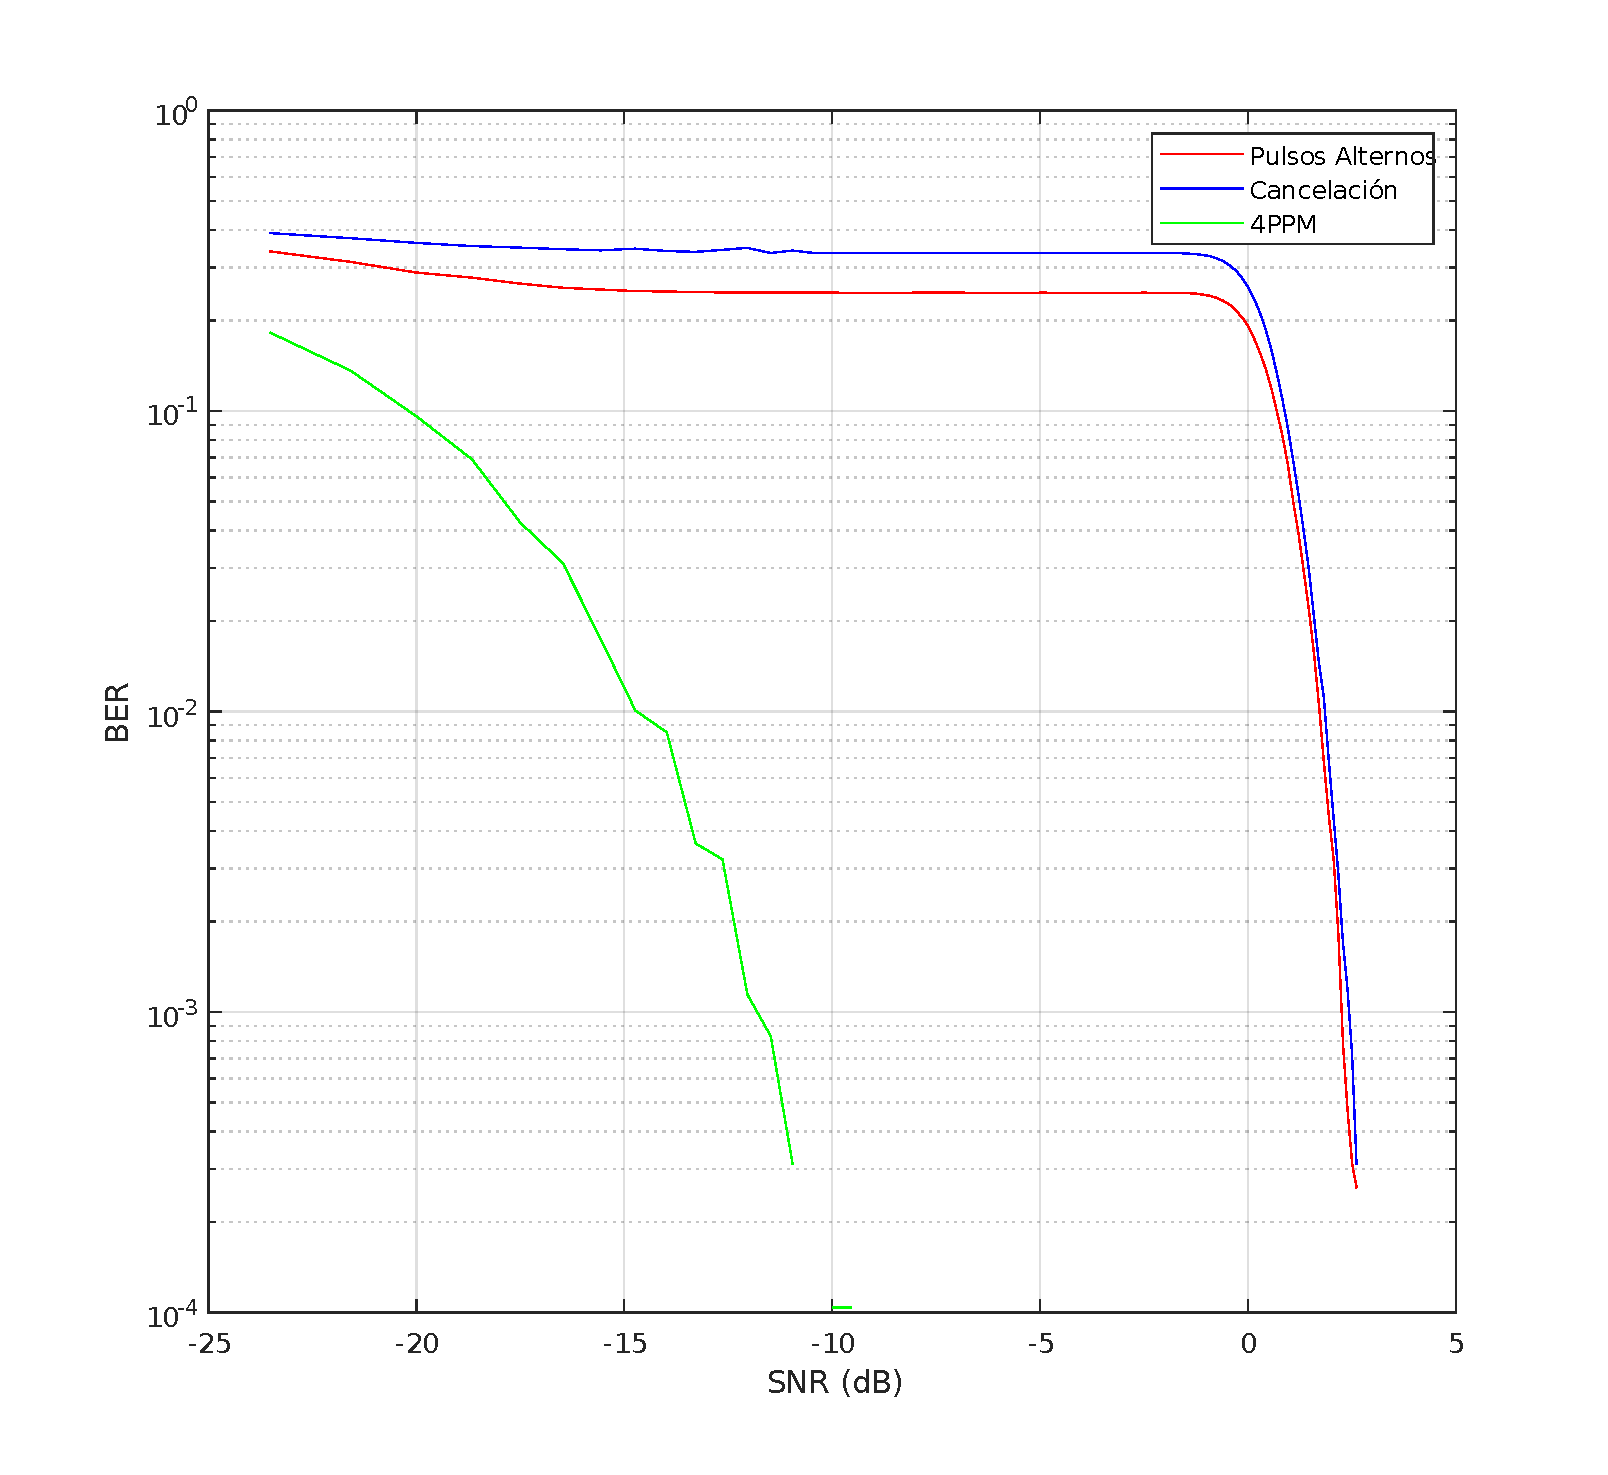
\includegraphics[scale=0.5]{./figuras/Soft.pdf}
    \caption{\small{Sistema \textit{Soft-decoding}.}}
    \label{soft-decoding}%
\end{figure}

En la figura se comprueba que pulsos alternos y cancelación de pulsos tienen un 
funcionamiento parecido al contar con las mismas opciones y, lo más importante, que
el funcionamiento de 4-ppm es mejor. Esto se debe, como se ha explicado anteriormente,
a que las distancias entre los puntos son las diagonales. Por lo tanto,
este método incrementa el potencial del 
uso de \textit{soft-decoding} y su funcionamiento es muy óptimo. 

%Conclusión
Finalmente, se concluye que, mientras que \textit{hard-decoding} opera con un solo bit de 
información, \textit{soft-decoding} puede tomar un rango de valores de entrada. Esta 
información adicional es fundamental para tener mejores estimaciones de los datos
originales.

En la línea de aumentar el rango de valores de entrada se trabaja con juntar 
\textit{soft-decoding} con el Algoritmo de Viterbi.


\subsection{Algoritmo de Viterbi}
El algoritmo de Viterbi es un algoritmo de programación dinámica que permite hallar 
la secuencia más probable (el llamado camino de Viterbi) que produce 
una secuencia observada, especialmente en el contexto de fuentes de información 
de Márkov.

En el trabajo se aplica el algoritmo de Viterbi en función del pasado, es decir, 
otorgandole memoria al sistema. Esto se usa para ampliar el rango de valores posibles, 
pero sobre todo, para que el número de opciones descartadas sea relevante en relación a
las opciones totales.

% Comentar que Viterbi va ligado a soft-decoding
Este sistema de decisión no es independiente, es decir, cuando se le otorga dicha 
memoria al sistema y se descartan las opciones no probables hay que elegir entre las
opciones que sí son posibles. Esta elección se realiza con el método 
\textit{soft-decoding} ampliando la fórmula bidimensional a el número de puntos que 
nos proporcine la memoria. Por lo tanto, se puede pensar que cuantos más pasados 
se tengan más robusto será el sistema. Sin embargo, mirar al pasado requiere de mucha
complejidad y de retardos de tiempo a la hora de calcular la distancia euclídea con 
tantos puntos. Por ello, hay que encontrar una solución de compromiso para que la mejora
sea significante y la complejidad no sea excesiva. En este trabajo vamos a quedarnos 
con un pasado.

En la aplicación de este método en nuestros sistemas de señalización hay bastantes 
diferencias entre ellos. Lo más importante es que no es útil aplicar este algoritmo para 
el esquema 4-PPM porque mirar el cuarteto anterior no tiene ningún impacto en el 
cuarteto actual ya que esta codificación no presenta restricciones entre la 
transmisión de cuartetos.

En el esquema pulsos alternos la aplicación del algoritmo de Viterbi si tiene sentido,
sin embargo, al mirar un pasado sólo se descartan dos opciones de las nueve posibles 
que tendría este esquema si no se usara Viterbi. Por esto, la mejora en cuanto a 
robustez que se presenta no es muy significativa respecto al método \textit{soft-decoding}
sin Viterbi del apartado anterior.

Para el esquema cancelación de pulsos usar el algoritmo de Viterbi es más eficaz que 
en el caso anterior. Esto es debido a que en este caso se descartan cuatro opciones de 
las nueve posibles por lo que la tiene un gran impacto en cuanto a la mejora de 
robustez frente al ruido.

En la figura \ref{viterbi} se muestra el funcionamiento de pulsos alternos y de cancelación de pulsos
con este método de decicisón.

\begin{figure}[ht]
    \centering
    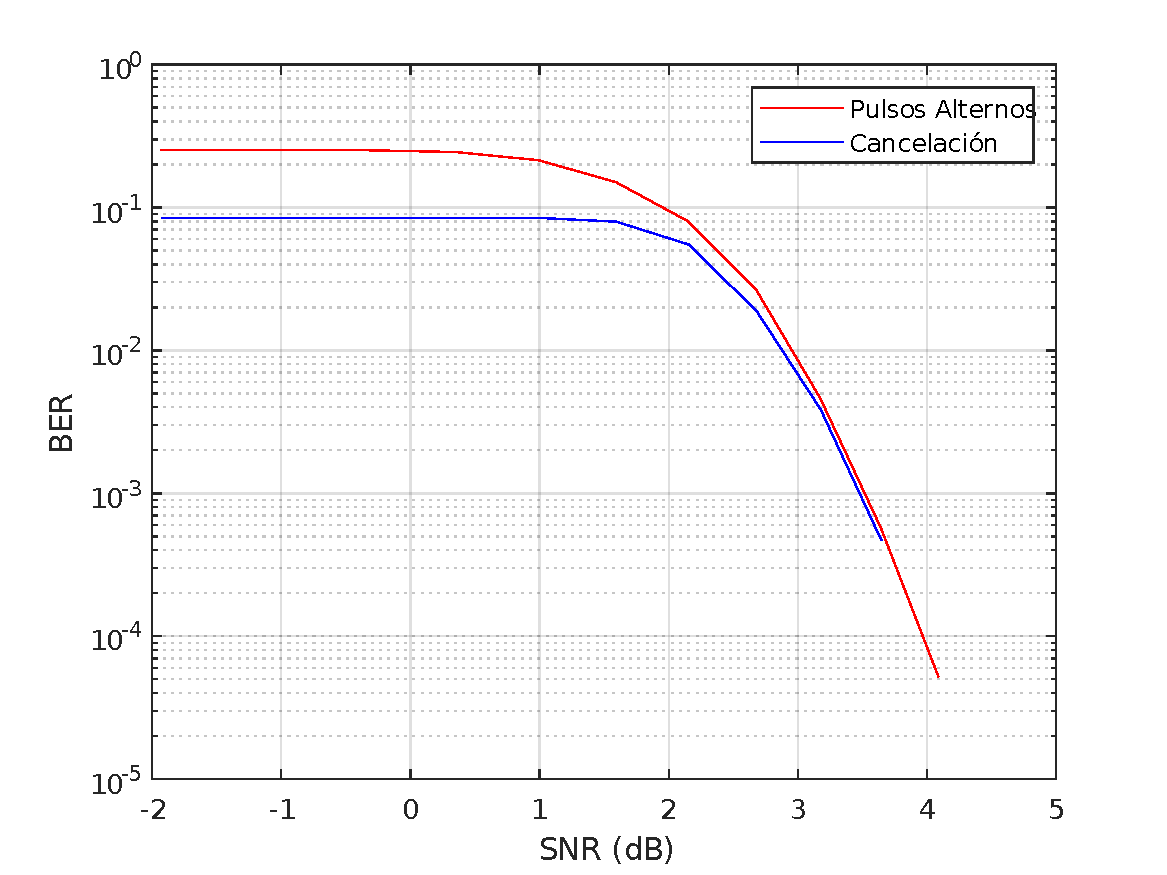
\includegraphics[scale=0.6]{./figuras/Viterbi.pdf}
    \caption{\small{Algoritmo de Viterbi.}}
    \label{viterbi}%
\end{figure}

Al analizar la gráfica se contempla que ambos esquemas mejoran respecto a la aplicación
de \textit{soft-decoding} sin Viterbi. Aunque tal y como se desarrollo anteriormente,
el uso de este algoritmo tiene más efecto en el esquema cancelación de pulsos llegando
a cambiar las tornas en cuanto a cuál de los dos es más robusto frente al ruido.


\subsection{Comparativa entre los sistemas de decisión}
A continuación, se va a comparar la tasa de error de bit (BER) de los distintos esquemas de decisión, para cada esquema 
de codificación, en función de la relación señal a ruido (SNR), que varia con la distancia (disminuyendo la 
amplitud de la señal), para verificar la mejora que se produce entre cada sistema de decisión.

La figura \ref{alternos} muestra una comparativa de los esquemas bajo 
la codificación de pulsos alternos.

\begin{figure}[ht]
    \centering
    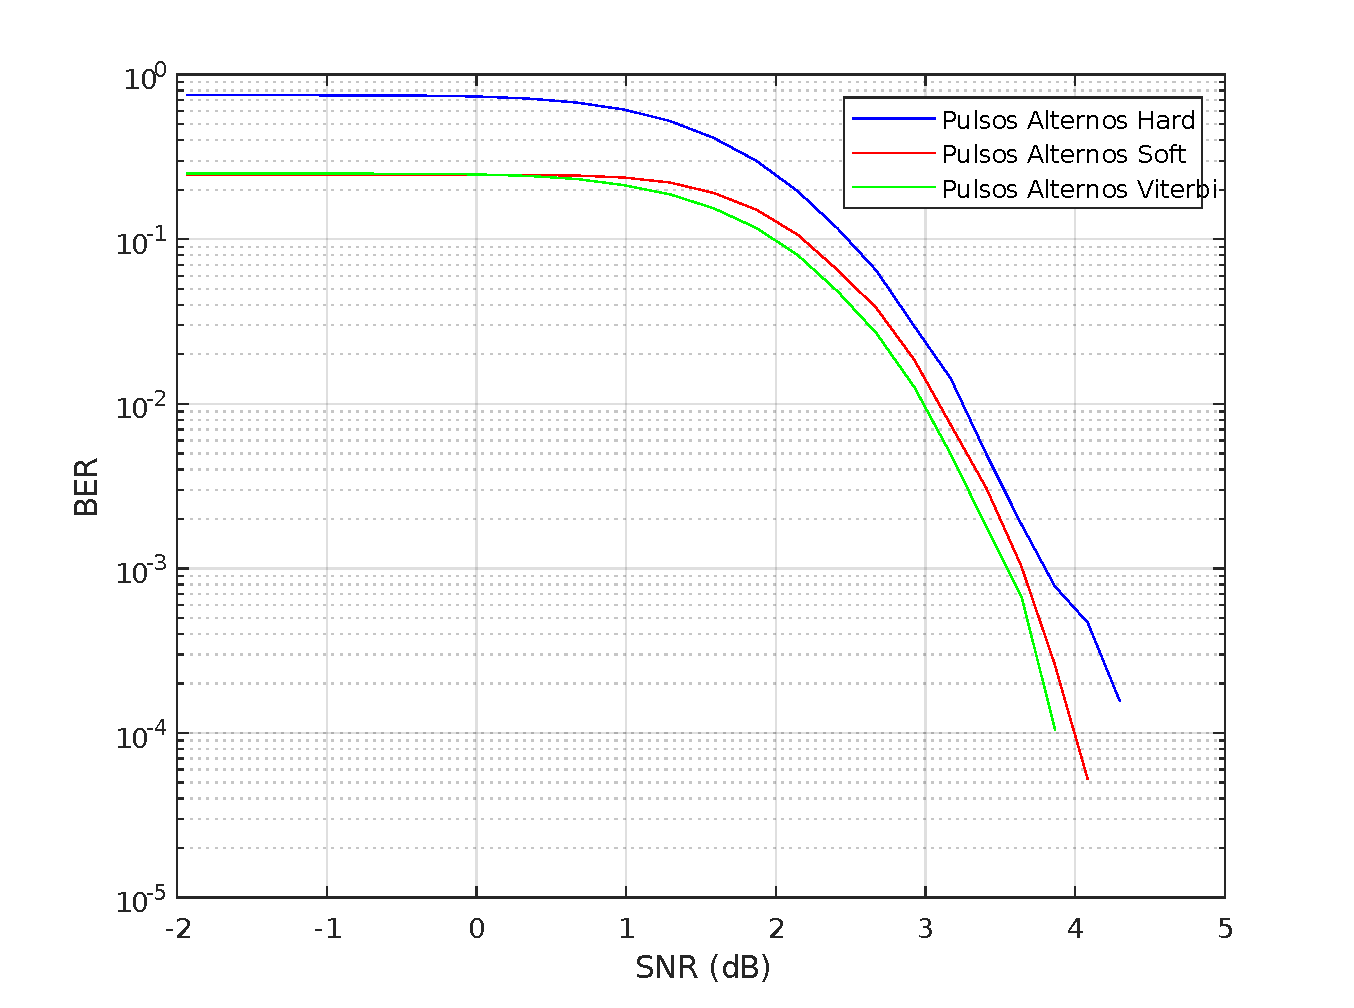
\includegraphics[scale=0.6]{./figuras/alternos.pdf}
    \caption{\small{Sistemas de decisión con pulsos alternos.}}
    \label{alternos}%
\end{figure}

Se observa que para pulsos alternos, la principal mejora se nota con la aplicación 
de soft-decoding o Viterbi. El funcionamiento de Viterbi es levemente mejor porque 
aplicando Viterbi con un pasado solo se descartan dos opciones de nueve posibles por lo 
que no sale a relucir su máximo potencial. 

La figura \ref{cancelacion} muestra una comparativa de los esquemas bajo 
la codificación de cancelación de pulsos.

\begin{figure}[ht]
    \centering
    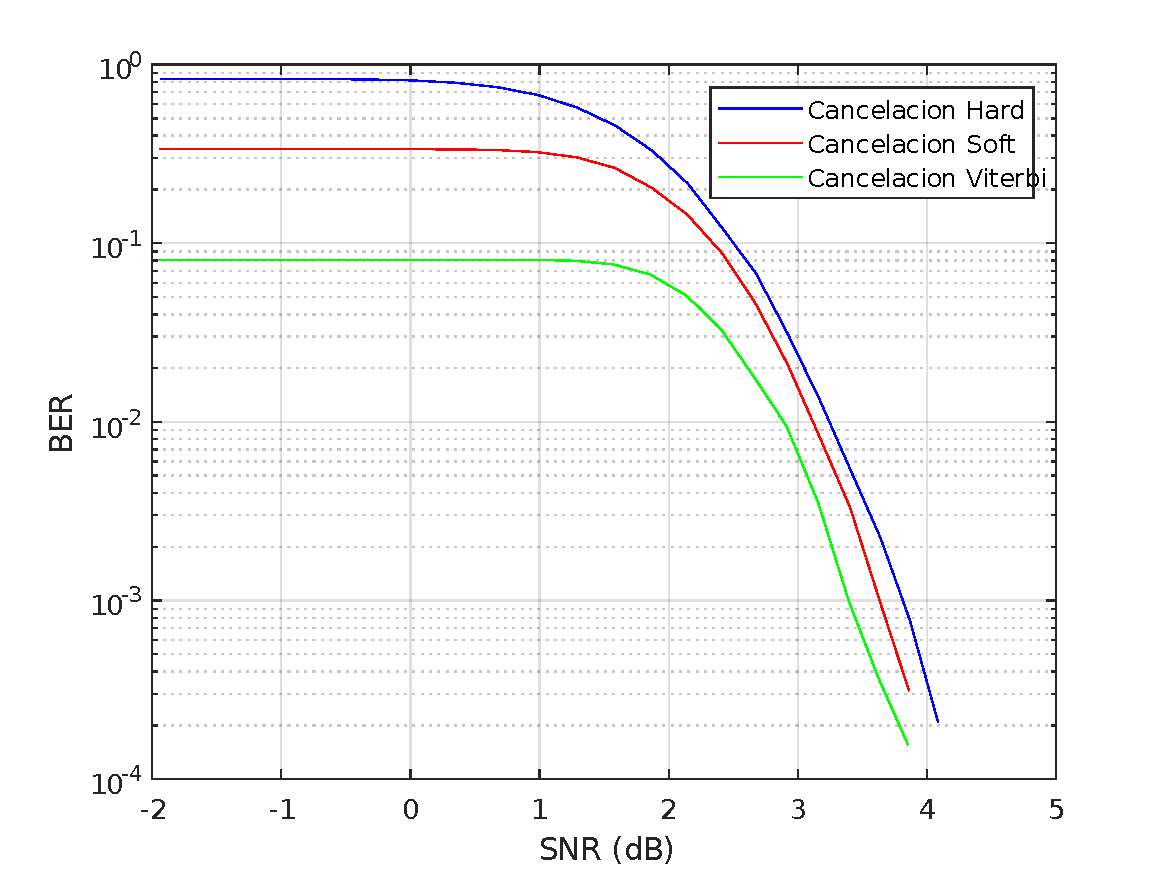
\includegraphics[scale=0.6]{./figuras/cancelacion.pdf}
    \caption{\small{Sistemas de decisión con cancelación de pulsos.}}
    \label{cancelacion}%
\end{figure}

Se comprueba que para cancelación de pulsos la aplicación del algoritmo de Viterbi 
es muy importante ya que, como se comentó en el apartado anterior, se descartan más 
opciones al mirar un pasado, concretamente se descartan cuatro de nueve opciones.

La figura \ref{4ppm} muestra una comparativa de los esquemas bajo 
la codificación 4-PPM.

\begin{figure}[ht]
    \centering
    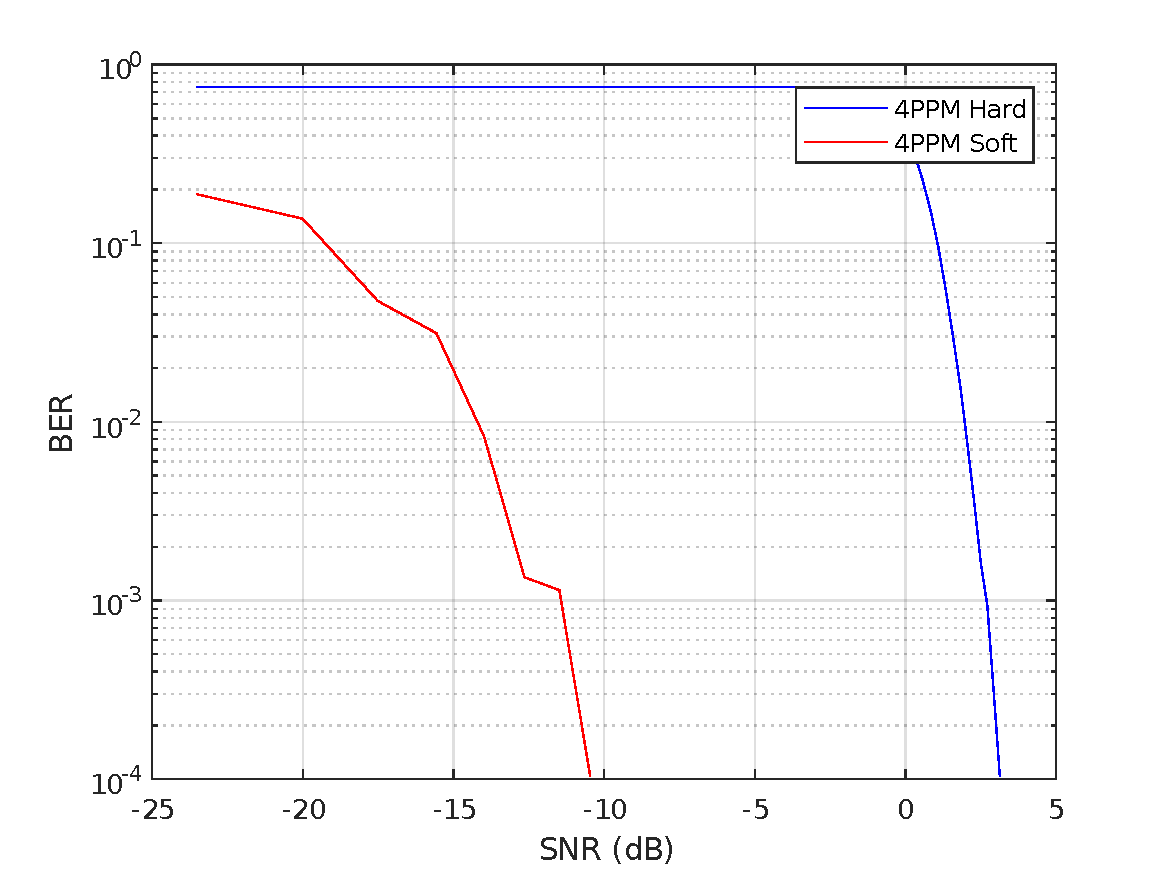
\includegraphics[scale=0.6]{./figuras/4ppm.pdf}
    \caption{\small{Sistemas de decisión con 4-PPM.}}
    \label{4ppm}%
\end{figure}

Se verifica que para 4ppm el uso de soft-decoding implica una gran mejora debido a 
la posibilidad de buscar el bit mayor ya que solo se recibe un '1' por cuarteto de bits.

\subsection{Conclusiones}
Finalmente, para concluir este apartado se muestra una gráfica comparativa de los 
tres esquemas de señalización con el sistema de deicisón que mejores prestaciones ofrece
a cada uno de ellos.

\begin{figure}[ht]
    \centering
    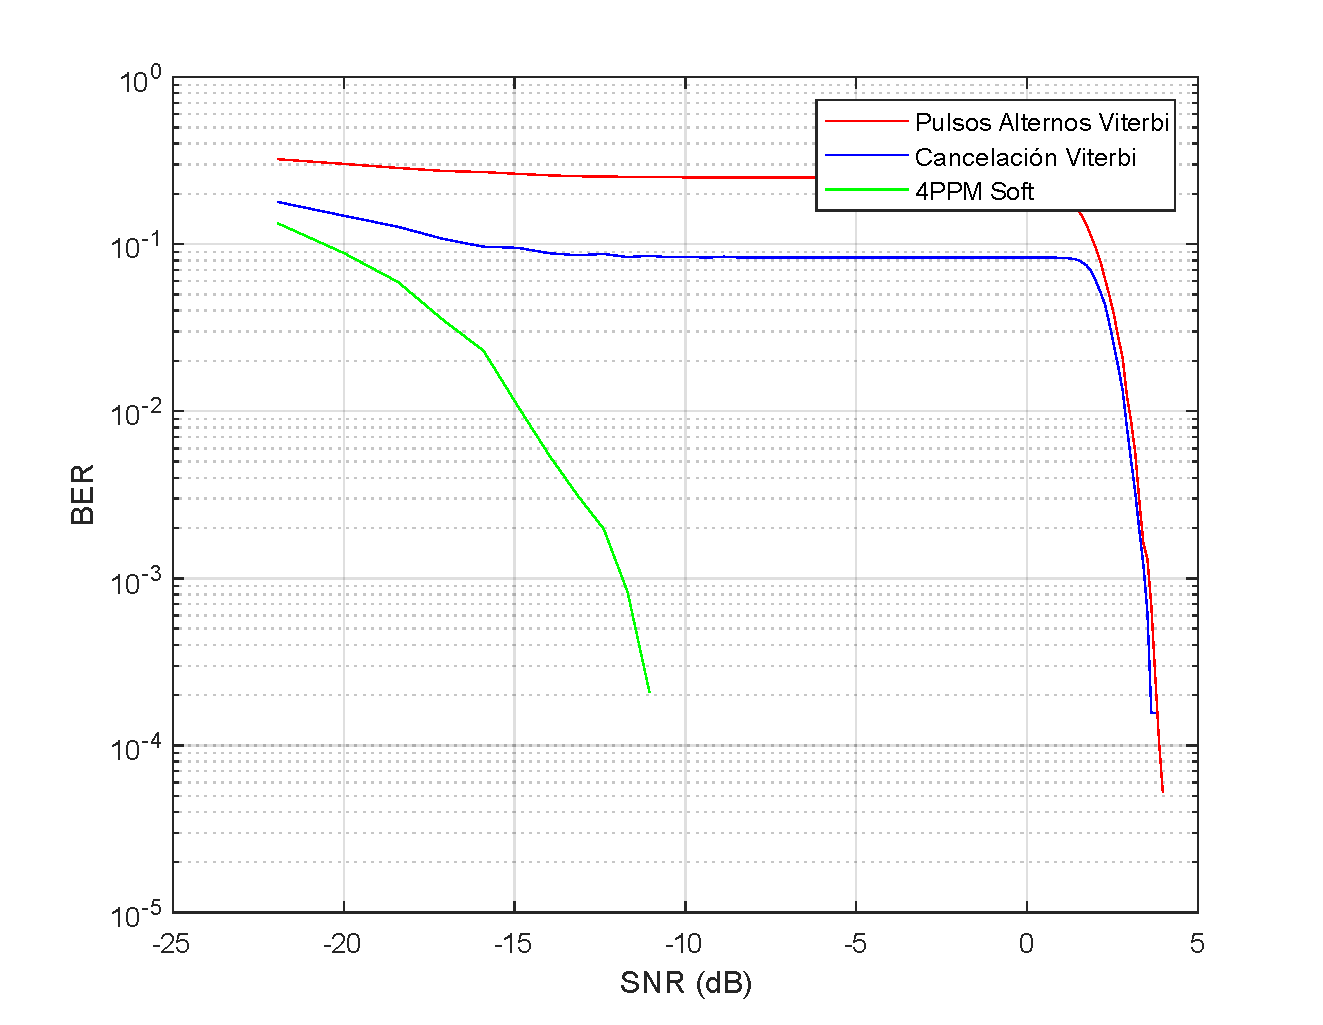
\includegraphics[scale=0.6]{./figuras/Comparativa.pdf}
    \caption{\small{Comparativa de los esquemas de codificación con su mejor sistema de deicisón.}}
    \label{comparativa}%
\end{figure}

Por tanto el mejor esquema de codificación en cuanto a robustez es 4-PPM con 
\text{soft-decoding}.

[TERMINAR DE CERRAR EL CAPÍTULO]

\chapterend{}
